%% to print two columns 
% \documentclass[tmptwocolumn, logo]{bioRxiv}

%% to print for review
\documentclass[submit, linenum, logo]{bioRxiv}

\usepackage{authblk}
\usepackage[utf8]{inputenc}
\usepackage[T1]{fontenc}%coding of the font
\usepackage{times}
\usepackage{bm}
\usepackage[english]{babel}
\usepackage{microtype}
\DisableLigatures[f]{encoding = *, family = * }
\usepackage{lmodern,booktabs,graphicx,siunitx,paralist,multirow}
\newcommand{\SIadj}[2]{\SI[number-unit-product={\text{-}}]{#1}{#2}}
\usepackage[labelfont=bf]{caption}
\usepackage{lipsum}
\usepackage{float}
\usepackage{placeins}
\usepackage{subfig}
\usepackage{MnSymbol,bbding,pifont}
\usepackage{bookmark}
\hypersetup{
    pdftitle={You can find this title in documentPreamble.tex},
    pdfauthor={First Author et al.},
    pdfsubject={Title of article},
    pdfkeywords={Key word 1, Key word 2, Key word 3},
    bookmarksnumbered=true,     
    bookmarksopen=true,         
    bookmarksopenlevel=5,       
    %colorlinks=true,       
    pdfstartview=Fit,           
    pdfpagemode=UseOutlines,    % this is the option you were lookin for
    pdfpagelayout=TwoPageRight
}

\usepackage[acronym,shortcuts=ac, nomain]{glossaries-extra}
\glsdisablehyper

% \usepackage[nolists,tablesfirst]{endfloat}

\usepackage{csquotes}
\usepackage{textcomp}
\usepackage{attachfile}
\usepackage[export]{adjustbox}
\usepackage[figure,table]{totalcount}
% \setlength{\parindent}{0in}
\graphicspath{{./figures/}}
% \DeclareGraphicsExtensions{.pdf}
\DeclareUnicodeCharacter{03C0}{$\pi$}

%!TEX root = manuscript.tex
\ExecuteBibliographyOptions{
  , backref=false
  , abbreviate=true
  , uniquename=false % this make Hoffman M and Hoffman Michael the same author
  , giveninits=true
  , terseinits=false % this remove the period in abbreviated first names
  , maxcitenames = 2
  , uniquelist=false
  , maxbibnames = 99
  , minbibnames = 3
  , doi=false
  , isbn=false
  , eprint=false
  , sortcites = false
  , autocite = superscript
  , sorting = none
  , url=true
  , sortlocale=de_DE
  , date=year
  , useprefix=true%this fix dutch names
  , hyperref=auto
  , defernumbers=true
}

\DeclareNameAlias{sortname}{family-given}

\AtEveryBibitem{%
	\clearfield{note}%
	\clearfield{url}%
	\clearfield{urldate}
	\clearfield{urlyear}%
    \clearfield{urlmonth}%
    %\clearfield{pages}%
    %\clearfield{volume}%
    \clearfield{number}%
    \clearfield{note}%
    \clearfield{month}%
    \clearfield{day}%
    % \clearfield{title}%
}
\AtEveryBibitem{\clearlist{language}}

\defbibenvironment{bibliography}
  {\begin{enumerate}}
  {\end{enumerate}}
  {\item}

\addbibresource{./library.bib}
\renewbibmacro{in:}{%
  \ifentrytype{article}{}{\printtext{\bibstring{in}\intitlepunct}}}
%\AtNextBibliography{\verysmall}

\addbibresource{library.bib}
\renewcommand*{\thesection}{\arabic{section}}
\renewcommand*{\thesubsection}{\thesection.\arabic{subsection}}
\renewcommand*{\thesubsubsection}{\thesubsection.\arabic{subsubsection}}
\setcounter{secnumdepth}{0} % this allow to avoid numbered sections
\let\subsectionautorefname\sectionautorefname
\let\subsubsectionautorefname\sectionautorefname
\usepackage{cleveref}
% \renewcommand{\autoref}[1]{\cref{#1}}
% \renewcommand{\Autoref}[1]{\Cref{#1}}
% \Autoref is for the beginning of the sentence
\let\orgautoref\autoref
\providecommand{\Autoref}[1]{%
\def\equationautorefname{Equation}%
\def\tableautorefname{Table}%
% \def\chapterautorefname{Chapter}%
%\def\figureautorefname{Figure}%
% \def\subfigureautorefname{Figure}%
% \def\sectionautorefname{Section}%
% \def\subsectionautorefname{Section}%
\orgautoref{#1}}
% \autoref is used inside the sentence to produce Fig., and Eq. for figures, subfigures, and equations
\renewcommand{\autoref}[1]{%
\def\equationautorefname{Eq.}%
%\def\figureautorefname{Figure}%
%\def\subfigureautorefname{Figure}%
% \def\sectionautorefname{Sec.}%
% \def\subsectionautorefname{Sec.}%
% \def\subsubsectionautorefname{Sec.}%
\orgautoref{#1}}
\usepackage{makecell}
% \renewcommand{\cite}[1]{\supercite{#1}}
% \renewcommand{\citep}[1]{\supercite{#1}}

%%%%%%%%%%%%%%%% list of figures
%\addto\captionsenglish{%
  %\renewcommand\listfigurename{}}
% \renewcommand{\cftfigdotsep}{\cftnodots} % no dots
% \renewcommand{\cftdotsep}{\cftnodots}

\cftpagenumbersoff{chapter}
\cftpagenumbersoff{section}
\cftpagenumbersoff{subsection}
\cftpagenumbersoff{subsubsection}
\cftpagenumbersoff{figure} % no page numbers
\setlength{\cftfigindent}{0.5em}
\setlength{\cftfignumwidth}{1.5em} 

%\makeatletter
%\renewcommand{\fnum@figure}[1]{\figurename\ \thefigure} % remove the : after number
%\renewcommand{\fnum@figure}[1]{\thefigure} % remove the : after number
%\makeatother

%%%%%%%%%%%%%%%%%%%%%%%%%%%%%%%%
\usepackage{newfloat}

\DeclareFloatingEnvironment[%
        name={Figure}, %
        placement=H, %
        listname={Main figure legends}%
    ]{myfigure}
\renewcommand{\thefigure}{\arabic{figure}}

\DeclareFloatingEnvironment[%
        name={Figure}, %
        placement=H, %
        listname={}%
    ]{supfigure}

\renewcommand{\thesupfigure}{S\arabic{supfigure}}

\DeclareFloatingEnvironment[
        name={Video}, %
        placement=H, %
        listname={Supplementary video legends}%
    ]{supvideo}
\renewcommand{\thesupvideo}{S\arabic{supvideo}}

%% create a counter for supplementary equations
\newcounter{my_supplementary_equation}
\makeatletter
\@addtoreset{equation}{my_supplementary_equation}
\makeatother
%!TEX root = manuscript.tex
\ExecuteBibliographyOptions{
  , backref=false
  , abbreviate=true
  , uniquename=false % this make Hoffman M and Hoffman Michael the same author
  , giveninits=true
  , terseinits=false % this remove the period in abbreviated first names
  , maxcitenames = 2
  , uniquelist=false
  , maxbibnames = 99
  , minbibnames = 3
  , doi=false
  , isbn=false
  , eprint=false
  , sortcites = false
  , autocite = superscript
  , sorting = none
  , url=true
  , sortlocale=de_DE
  , date=year
  , useprefix=true%this fix dutch names
  , hyperref=auto
  , defernumbers=true
}

\DeclareNameAlias{sortname}{family-given}

\AtEveryBibitem{%
	\clearfield{note}%
	\clearfield{url}%
	\clearfield{urldate}
	\clearfield{urlyear}%
    \clearfield{urlmonth}%
    %\clearfield{pages}%
    %\clearfield{volume}%
    \clearfield{number}%
    \clearfield{note}%
    \clearfield{month}%
    \clearfield{day}%
    % \clearfield{title}%
}
\AtEveryBibitem{\clearlist{language}}

\defbibenvironment{bibliography}
  {\begin{enumerate}}
  {\end{enumerate}}
  {\item}

\addbibresource{./library.bib}
\renewbibmacro{in:}{%
  \ifentrytype{article}{}{\printtext{\bibstring{in}\intitlepunct}}}
%\AtNextBibliography{\verysmall}

\renewcommand{\topfraction}{0.95}%.7
\renewcommand{\textfraction}{0.05}%.3
\renewcommand{\floatpagefraction}{0.99}%.5
\setglossarystyle{long}
\newglossary[slg]{symbolslist}{syi}{syg}{List of Symbols}
%Remove the dot at the end of glossary descriptions
\renewcommand*{\glspostdescription}{}
%\renewcommand*{\glstextformat}[1]{\textcolor{black}{#1}}

\setabbreviationstyle[acronym]{long-short-desc}
\newabbreviation{MSA}{MSA}{my super acronym}
\newabbreviation{EEG}{EEG}{electroencephography}
\newabbreviation{AM}{AM}{amplitude modulation}
\newabbreviation{ANOVA}{ANOVA}{analysis of variance}
\newabbreviation{LME}{LME}{linear mixed-effects}


\newcommand\wordcount{\input{|"texcount -inc -sum -0 -template={SUM} \jobname.tex"}}
%TC:macro \cite [option:ignore,ignore]
\begin{document}
%TC:ignore
\leadauthor{The Lead Author name}
\title{My very cool paper}
\shorttitle{Cool paper}

\author[1, 2]{Author 1 \orcidlink{0000-0000-0000-0000}}
\author[1, 3]{Author 2 \orcidlink{0000-0000-0000-0001}}
\affil[1]{My Department, 0 Street Name, Best University in the world, Postal code, Australia}
\affil[2]{My Department 2, 0 Street Name 2, Almost Best University in the world, Postal code, Australia}
\affil[3]{My Department 3, 0 Street Name 3, Not the Best University in the world, Postal code, Australia}


\date{}
\maketitle
%TC:endignore

%TC:ignore
\begin{leadcontact}
author1@myuni.org (A1) % author email and initials
\end{leadcontact}

\begin{corrauthor}
author1@myuni.org (A1), author2@myuni.org (A2)
\end{corrauthor}

%TC:endignore

%TC:ignore
\begin{abstract}
 %!TEX root = manuscript.tex
\section*{Abstract}
\label{sec:abstract}
Over several years .... 

\lipsum[1-2]
\end{abstract}
%TC:endignore

%TC:ignore
\begin{keywords}
Key word 1 | Key word 2 | Key word 3 
\end{keywords}
%TC:endignore

%TC:ignore
\phantomsection\label{sec:title}
\addcontentsline{toc}{chapter}{My very cool paper}
%TC:endignore
\newrefsection
\section*{Introduction}
\phantomsection\label{sec:Introduction}
\addcontentsline{toc}{section}{Introduction}
\glsresetall

This article investigate a super model \citep{struttTheorySound1877}. 
You can use acronyms defined in acronyms.tex, for example \acp{MSA}.
Text continue ...
Another acronym (defined in acronym.tex) \ac{AM}.

An example figure 

\begin{figure*}
	\centering
	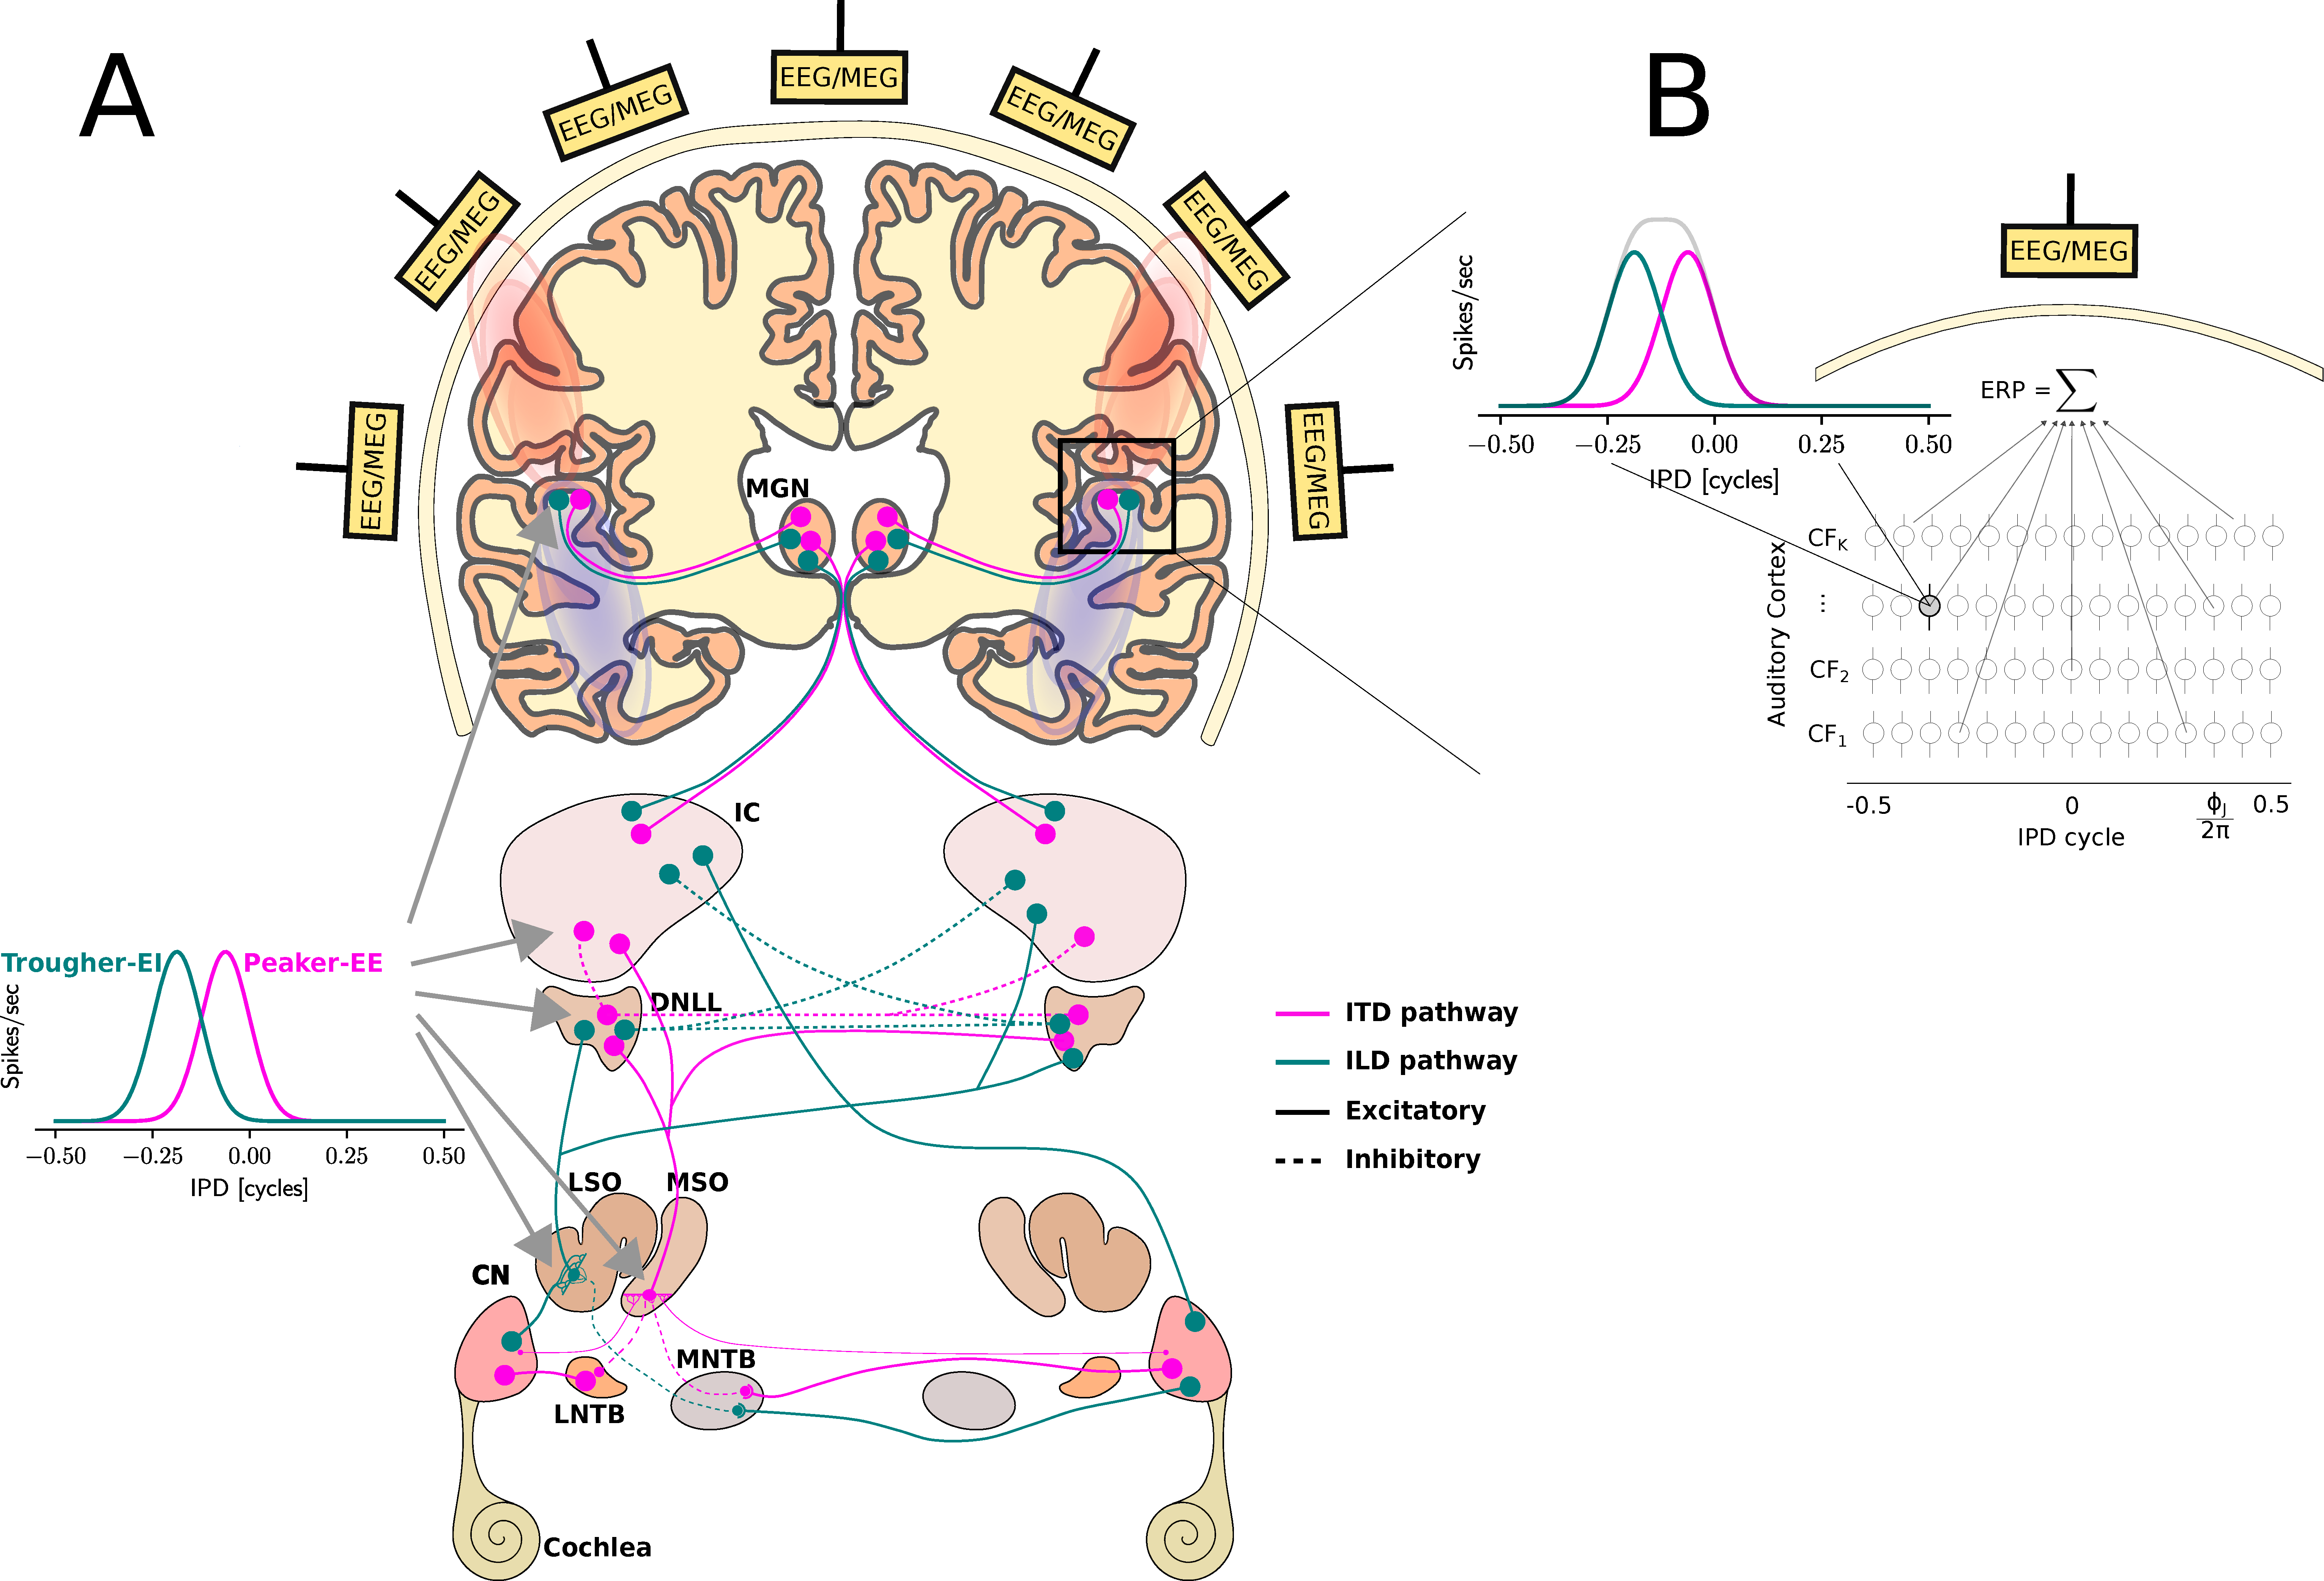
\includegraphics[width=16cm]{./figures/figure_example.pdf} % your figure should be in figure folder
	\caption{
	\textbf{\color{Black}Figure experiment heading.}
	\textbf{A}, this figure shows a model from Undurraga et al. 2023
	\textbf{B}, another panel
	}
	\label{fig:example_figure_0}
\end{figure*}

\lipsum[1-4]
\section*{Methods}
\phantomsection\label{sec:methods}
\addcontentsline{toc}{section}{Methods}

\subsection*{Resource Availability}
\phantomsection\label{subsec:resources}
\addcontentsline{toc}{subsection}{Resource Availability}

\subsubsection*{Lead contact}
\phantomsection\label{subsubsec:contact}
\addcontentsline{toc}{subsubsection}{Lead contact}

Further information and requests for resources and data should be directed to and will be fulfilled by the lead contact, Lead.Contact.Name (lead.contact@email.com). 

\subsubsection*{Materials availability}
\phantomsection\label{subsubsec:materials}
\addcontentsline{toc}{subsubsection}{Materials availability}
The current study has not (or maybe it did) generated any new material.

\subsubsection*{Data and code availability}
\phantomsection\label{subsubsec:data}
\addcontentsline{toc}{subsubsection}{Data and code availability}
Complete data sets as well as source code used to generate all figures and statistical analyses have been deposited at \href{https://google.com}{My data repo} and \href{https://gitlab.com/}{Gitlab} and are publicly available as of the date of publication. 
The instructions to reproduce all results are also provided there.


\subsection*{Experimental model and subject details}
\phantomsection\label{subsec:Expt1_Subjects}
\addcontentsline{toc}{subsection}{Experimental model and subject details}
A million participants took part in this study.

\subsection*{Method details}
\phantomsection\label{subsec:method_details}
\addcontentsline{toc}{subsection}{Method details}

\subsubsection*{Stimuli}
\phantomsection\label{subsec:stimuli}
\addcontentsline{toc}{subsubsection}{Stimuli}
Stimuli consisted of ...


\subsubsection*{EEG recordings}
\phantomsection\label{subsec:eeg_recording}
\addcontentsline{toc}{subsubsection}{EEG recordings}
\Ac{EEG} recordings were obtained from ... 

\subsubsection*{\ac{EEG} analyses}
\phantomsection\label{subsec:eeg_data_analyses}
\addcontentsline{toc}{subsubsection}{EEG analyses}

The processing pipeline included several steps.... 


\subsubsection*{Behavioural experiment}
\phantomsection\label{subsec:anchoring_behavioural}
\addcontentsline{toc}{subsubsection}{Behavioural experiment}
In order to assess the perceptual ...

\lipsum[1-6]


\subsubsection*{Statistical analyses}
\phantomsection\label{subsubsec:statistics}
\addcontentsline{toc}{subsubsection}{Statistical analyses}
\Ac{ANOVA} were carried out be means of \ac{LME} models for which the factor subject was set as random ....  
See \autoref{eq:eq1}


\begin{align}
	\begin{split}
	\label{eq:eq1}
	y & = \beta_0 + x + \\
	&  \beta_1 e^{-\frac{\left( \beta_1 \right)}{\tau}} \\
	\end{split}
\end{align}


\noindent With $\beta_0$ ...


\section*{Results}
\phantomsection\label{sec:results}
\addcontentsline{toc}{section}{Results}

\subsection*{A super cool experiment}
\phantomsection\label{subsec:a_super_cool_experiment}
\addcontentsline{toc}{subsection}{A super cool experiment}

In this experiment using \ac{MSA} we found ... 
The value in international units is \SI{10}{\ms}. 
You can also use \SI{100}{\Hz}. 


%TC:ignore
\begin{figure}
	\centering
	% \includegraphics[width=16cm]{./figures/figure_1.pdf} % your figure should be in figure folder
	\includegraphics[width=8.0cm]{example-image-a}
	\caption{
	\textbf{\color{Black}Figure experiment heading.}
	\textbf{A}, This figure shows (\acs{MSA}) \citep{undurragaNeuralRepresentationInteraural2016}.
	See also \autoref{fig:example_figure_2}.
	}
	\label{fig:example_figure_1}
\end{figure}

Also we found that ....

\lipsum[1-4]

\begin{figure}
	\centering
	% \includegraphics[width=16cm]{./figures/figure_1.pdf} % your figure should be in figure folder
	\includegraphics[width=8.0cm]{example-image-b}
	\caption{
	\textbf{\color{Black}Another figure experiment heading.}
	\textbf{A}, This figure shows something different than \autoref{fig:example_figure_1}.
	}
	\label{fig:example_figure_2}
\end{figure}

Finally 

\lipsum[1-4]

%TC:endignore

%!TEX root = manuscript.tex
\section*{Discussion}
\phantomsection\label{disc:Discussion}
\addcontentsline{toc}{section}{Discussion}

My experiments demonstrated that ....

\lipsum[1-4]

%TC:ignore
%This document has \wordcount words.
%TC:endignore

%TC:ignore
\section*{Acknowledgments}
\phantomsection\label{sec:acknowledgments}
\addcontentsline{toc}{section}{Acknowledgments}
This study was supported by my nice grant (Grant No. XXX-XXX).
The authors thank Someone that helped (if anyone).
\section*{Author contributions}
\phantomsection\label{sec:authorcontributions}
\addcontentsline{toc}{section}{Author contributions}
A1 and A2 conceptualized and designed the experiments.
A1 performed the neurophysiological experiments.
A2 performed the behavioural experiment.
A1 and A2 analysed the neurophysiological data.
A1 and A2 wrote the manuscript with the input from all authors.

\section*{Declaration of interests}
\phantomsection\label{sec:declaration}
\addcontentsline{toc}{section}{Declaration of interests}
The authors declare no competing interests (or maybe you do).


% \newpage
% \phantomsection\label{sup:Main figure legends}
% \addcontentsline{toc}{section}{Main figure legends}
% {%
% \let\oldnumberline\numberline%
% \renewcommand{\numberline}{\textbf\myfigurename~\oldnumberline}%
% \vspace*{-3cm}
% \listoffigures%
% }


% \newpage
% \subsection*{}
% \phantomsection\label{sup:Supplementary video legends}
% \addcontentsline{toc}{section}{Supplementary video legends}
% {%
% \let\oldnumberline\numberline%
% \renewcommand{\numberline}{\textbf\supvideoname~\oldnumberline}%
% \listofsupvideos
% }


\newpage
\subsection*{References}
\printbibliography[heading=none]
\endrefsection


\newpage

\newrefsection
\defbibenvironment{supbibliography}
  {\list
     {\printtext[labelnumberwidth]{%
        \printfield{prefixnumber}%
        \printfield{labelnumber}}}
     {\setlength{\labelwidth}{\labelnumberwidth}%
      \setlength{\leftmargin}{\labelwidth}%
      \setlength{\labelsep}{\biblabelsep}%
      \addtolength{\leftmargin}{\labelsep}%
      \setlength{\itemsep}{\bibitemsep}%
      \setlength{\parsep}{\bibparsep}}%
      \renewcommand*{\makelabel}[1]{\hss##1}}
  {\endlist}
  {\item}
\DeclareFieldFormat{labelnumberwidth}{\mkbibbrackets{#1}}

\newpage
%  CONFIGURE NEW SINGLE-PAGE FORMAT 
\onecolumn % go back to one column
\fancyhead{} % make sure we get no headers
\renewcommand{\floatpagefraction}{0.1}
\lfoot[\bSupInf]{\dAuthor}
\rfoot[\dAuthor]{\cSupInf}
\newpage

\captionsetup*{format=largeformat} % make figure legend slightly larger than in the paper

\newpage
\section*{}

\begin{supfigure}
	\centering
	% \includegraphics[width=14.0cm]{./figures/figure_1S.pdf}
	\includegraphics[width=14.0cm]{example-grid-100x100pt}
	\caption{
	\textbf{\color{Black}Supplementary figure 1}
	\textbf{A} \lipsum[1-2]
    }
	\label{fig:sup_1}  
\end{supfigure}



\newpage
\newrefcontext[labelprefix=S]
\printbibliography[env=supbibliography]
\endrefsection

\newpage
%  CONFIGURE NEW SINGLE-PAGE FORMAT 
\onecolumn % go back to one column
\fancyhead{} % make sure we get no headers
\renewcommand{\floatpagefraction}{0.1}
\lfoot[\bSupInf]{\dAuthor}
\rfoot[\dAuthor]{\cSupInf}
\newpage

\captionsetup*{format=largeformat} % make figure legend slightly larger than in the paper
%\setcounter{figure}{0} % reset figure counter for Supplementary Video Figures
%\setcounter{page}{1} % reset page count
%\makeatletter 
%\renewcommand{\thefigure}{SV\@arabic\c@figure} % make Figure legend start with Figure S
%\makeatother

%  MAIN TEXT 
\newpage
%\section*{}
%\phantomsection\label{sup:videos}
%\addcontentsline{toc}{section}{Supplementary Videos}

%\subsection*{Sources time course of ITD-FR and ASSR}
\phantomsection\label{sup:source_time}
\addcontentsline{toc}{subsection}{Sources time course of ITD-FR and ASSR}

\begin{supvideo}
% \renewcommand\figurename{Video}
\begin{minipage}{0.5\linewidth}
	\centering
	\begin{minipage}{.3\linewidth}
		\centering
		%\textattachfile[color=0 0 0]{./figures/Video_S1.mp4}{\textbf{Video SV1}}
	\end{minipage}\\%
 \end{minipage}
%
	\caption{
	\textbf{\color{Black}Vides.}
	\textbf{A}, My A video
	}
	\label{sv:sup_video_1}  
\end{supvideo}


%TC:endignore

\end{document}
